% Final report (main, ~6 pages) - FAI Group 22.
% Compile from this directory: pdflatex report && pdflatex report
% Figures come from `python run_evaluation.py report ... --report-dir Doc/report`.
% Every number below is taken from results/sweep_*/summary.csv; the per-cell tables with
% confidence intervals are in supplementary.tex.
\documentclass[11pt]{article}

\usepackage[margin=1in]{geometry}
\usepackage[utf8]{inputenc}
\usepackage[T1]{fontenc}
\usepackage{amsmath,amssymb,amsfonts}
\usepackage{booktabs}
\usepackage{graphicx}
\usepackage{microtype}
\usepackage{enumitem}
\usepackage{dsfont}
\usepackage{caption}
\usepackage[numbers,sort&compress]{natbib}
\usepackage[hidelinks]{hyperref}

\captionsetup{font=small,labelfont=bf}
\setlist{nosep,leftmargin=*}
\newcommand{\Reg}{\mathrm{Reg}}
\newcommand{\Eff}{\mathrm{Eff}}

\title{Learning to Bid Under a Budget: A Batched First-Price Ad Auction\\with Unknown Click Probabilities}
\author{Vivek Raj \and Anvit Aggarwal \and Eshaan Ashish Jaiswal \and Gella Naga Sai Krishna\\[0.3em]
\small CS329 Foundations of AI, Group 22 --- IIT Gandhinagar}
\date{}

\begin{document}
\maketitle
\vspace{-1.5em}

\begin{abstract}
Budget-constrained advertisers repeatedly buy impressions in a batched first-price auction: each round
they submit one bid per user, subject to a budget, without knowing how likely each user is to click.
With known click probabilities the best response is a $0$--$1$ knapsack, which we use to compute
reference equilibria (Tier~1). We then let one advertiser learn against fixed equilibrium opponents
(Tier~2) and let all advertisers learn at once (Tier~3). A shared evaluation harness measures regret,
equilibrium gap, allocation efficiency, profit and revenue over $30$ seeds with $95\%$ confidence
intervals, across $m\in\{2,3,5\}$ advertisers, $n\in\{5,\dots,50\}$ users, four budget levels and three
budget structures. Thompson sampling is the best learner in every Tier-2 cell (regret grows as
$T^{0.33}$ at $T=10^3$ and $T^{0.2}$ at $T=10^4$). When all advertisers learn, the market stays away
from equilibrium by an amount that grows with $m$, and most of that gap is already present with known
click probabilities. Scarce budgets cost efficiency through the equilibrium itself rather than by slowing learning.
\end{abstract}

% =====================================================================
\section{Introduction}
Online ad platforms sell many impressions at once to advertisers who have fixed budgets and do not
know in advance which users will click. Each advertiser has to decide which users to buy and how much
to pay for them, and can only learn a user's click rate by winning that user. Two literatures meet
here. Auction theory describes what budget-constrained bidders do at equilibrium when values are known,
and bandits with knapsacks~\citep{badanidiyuru2013bandits} and combinatorial
semi-bandits~\citep{chen2013combinatorial} describe how one agent learns under resource constraints.
We ask: \emph{how much do advertiser profit and allocation efficiency suffer when click probabilities
must be learned online, and how does that change when every advertiser learns at the same time?}

We relax one assumption at a time. \textbf{Tier~1} assumes known click probabilities and computes
best responses and equilibria. \textbf{Tier~2} gives one advertiser a bandit learner against opponents
fixed at the Tier-1 equilibrium, which is a stationary single-agent problem. \textbf{Tier~3} lets all
advertisers learn concurrently, so each faces a non-stationary market. Our contributions are
(i) an exact knapsack formulation of the per-round best response and its use as a learning oracle,
(ii) five budget-aware learners evaluated through one shared harness, and (iii) a $30$-seed study over
$48$ market sizes $(m,n,\kappa)$, three budget structures and two horizons. A live demo accompanies the
report (Section~\ref{sec:repro}).

% =====================================================================
\section{Model}\label{sec:model}
Advertisers $a_1,\dots,a_m$ compete for users $u_1,\dots,u_n$ over $T$ rounds. Advertiser $i$ gets a
click from user $j$ with unknown probability $f_{ij}\in[0,1]$, worth $v$ to it. In round $t$ it submits
integer bids $b^t_{ij}\in\{0,\dots,B_i\}$ with $\sum_j b^t_{ij}\le B_i$. On each user the highest
positive bid wins, ties are broken uniformly at random, and the winner pays its bid whether or not the
user clicks. A won impression produces a click $X^t_{ij}\sim\mathrm{Ber}(f_{ij})$. With $q_{ij}(b)$ the
probability that $i$ wins $u_j$ under profile $b$, the expected profit is
\begin{equation}
  p_i(b)=\textstyle\sum_{j} q_{ij}(b)\,\big(f_{ij}v-b_{ij}\big).
\end{equation}
\emph{Feedback.} Advertiser $i$ sees clicks only on users it won (semi-bandit feedback) and sees the
highest competing bid $c^t_{-i,j}=\max_{k\ne i} b^t_{kj}$ on every user.

\paragraph{Best response is a knapsack.} Fix the competing bids $c_{-i}$. Bidding exactly
$c_{-i,j}+1$ wins $u_j$ outright, and any lower positive bid wins nothing, ties aside. So the best
response chooses a set of users $x\in\{0,1\}^n$:
\begin{equation}\label{eq:knap}
  \max_{x}\ \sum_j \big(f_{ij}v-c_{-i,j}-1\big)x_j
  \quad\text{s.t.}\quad \sum_j (c_{-i,j}+1)\,x_j\le B_i ,
\end{equation}
a $0$--$1$ knapsack with integer weights, solved exactly by dynamic programming in $O(nB_i)$ time; the
bids are $b_{ij}=(c_{-i,j}+1)x_j$. With integer bids the cheapest win costs at least $1$, so under the
normalisation $v=1$ every item value $f_{ij}-c_{-i,j}-1$ is non-positive and nobody ever bids. All
experiments therefore use $v=5$, so that a win at price $1$ is profitable whenever $f_{ij}>0.2$.

\paragraph{Tier 1: reference equilibria.} The game is finite, so a mixed Nash equilibrium exists. We
compute a reference profile $b^*$ with best-response dynamics (each advertiser in turn plays
\eqref{eq:knap}) and fall back to fictitious play and, for small instances ($m\le3$, $n\le5$), support
enumeration. We also compute the omniscient planner's allocation $u_j\mapsto\arg\max_i f_{ij}$, which
upper-bounds welfare.

\paragraph{Tiers 2 and 3: learners.} Every learner keeps, per user, the number of won impressions
$N_j$ and clicks $s_j$, and solves \eqref{eq:knap} with $f_{ij}$ replaced by an index $\tilde f_j$
and $c_{-i}$ replaced by the competing bids observed in the previous round. Round~$1$ is a zero-bid probe
that reveals $c_{-i}$ at no cost.
\begin{itemize}
  \item \textbf{UCB}: $\tilde f_j=\min\{1,\ s_j/N_j+\sqrt{\alpha\ln t/N_j}\}$, and $\tilde f_j=1$ if
        $N_j=0$; $\alpha\in\{0.5,1,2\}$, default $2$.
  \item \textbf{Thompson sampling (TS)}: $\tilde f_j\sim\mathrm{Beta}(1+s_j,\ 1+N_j-s_j)$.
  \item \textbf{Greedy}: $\tilde f_j=s_j/N_j$ (no exploration bonus); \textbf{$\epsilon$-greedy}: as
        greedy, but with probability $\epsilon=0.1$ it buys a random feasible set.
  \item \textbf{Budget-paced}: for a single campaign budget shared across rounds, a UCB learner that
        subtracts a dual price $\lambda_t\,(c_{-i,j}+1)$ from each item value and raises $\lambda_t$ when
        spending runs ahead of the per-round rate, approximating the fluid LP of bandits with
        knapsacks~\citep{badanidiyuru2013bandits,agrawal2014bandits}.
\end{itemize}
In Tier~2 advertiser $a_1$ runs a learner and $a_{2..m}$ play $b^*_{-1}$. In Tier~3 all $m$ run the
same learner. As a Tier-3 control, \texttt{oracle\_br} gives every advertiser the true $f$ and has it
best-respond to last round's bids. This is simultaneous best-response dynamics with the learning removed,
and it separates the effect of concurrent adaptation from the effect of not knowing $f$.

% =====================================================================
\section{Experimental methodology}\label{sec:method}
\paragraph{Harness.} Every agent implements one interface (\texttt{get\_bid}, \texttt{observe},
\texttt{reset}) and is registered by name, so the same simulator runs all tiers. Each round, the
simulator collects bids, resolves the auction with the shared auction engine and returns feedback. An
infeasible bid vector is replaced by zeros. This happens only under cumulative budgets, when an agent
that does not track its campaign budget (fixed $b^*$ or a myopic learner) bids more than it has left,
and it effectively ends that agent's campaign; the paced agent never triggers it. Metrics are computed with the true
$f$, which the agents never see:
\begin{itemize}
  \item \textbf{Regret} $\Reg^{(i)}_T=\sum_t\big(p_i^*(c^t_{-i})-p_i(b^t)\big)$, where $p_i^*$ is the
        value of \eqref{eq:knap} against the competing bids actually played. We summarise its growth by the
        least-squares slope of $\log\Reg_t$ against $\log t$ for $t\ge T/10$; a slope below $1$ means
        sublinear regret ($0.5$ for $\sqrt T$-type, near $0$ for logarithmic).
  \item \textbf{Equilibrium gap} $\varepsilon_t=\max_i \max\{0,\ p_i^*(c^t_{-i})-p_i(b^t)\}$: how
        much the most dissatisfied advertiser could gain by deviating. Also $\|b^t-b^*\|_1$.
  \item \textbf{Efficiency} $\Eff_t=\frac1n\sum_j\sum_{i\in\arg\max_k f_{kj}}q_{ij}(b^t)$, the share of
        users won by their highest-value advertiser; platform revenue $\sum_{ij}q_{ij}b^t_{ij}$; welfare.
  \item \textbf{Price of learning}: the Tier-1 value of a metric minus its final value under learning.
\end{itemize}
``Final'' values average the last $10\%$ of rounds.

\paragraph{Instances and grid.} Click rates are drawn as $f_{ij}\sim\mathrm{Beta}(2,5)$ (mean $0.29$);
budgets are $B_i=\max(1,\mathrm{round}(\kappa n))$. The parameter grid consists of
$m\in\{2,3,5\}$, $n\in\{5,10,20,50\}$, and $\kappa\in\{0.1,0.25,0.5,1\}$ ($48$ cells), with
$30$ seeds per cell, horizon $T=10^3$, and Student-$t$ $95\%$ intervals. The realised tightness
$\kappa_i=B_i/\sum_j(c^*_{-i,j}+1)$ at $b^*$ lies between $0.10$ and $0.53$ on average, so the grid
spans scarce to moderate budgets. A long-horizon study uses $T=10^4$ on $m\in\{2,3\}$, $n\in\{10,20\}$,
$\kappa=0.5$.

\paragraph{Budget structures.} \emph{Canonical}: the budget resets every round. \emph{Discounted}: as
canonical, but round $t$ is weighted by $\gamma^{t-1}$ ($\gamma=0.999$). \emph{Cumulative}: one budget of
$\rho TB_i$ ($\rho=0.5$) for the whole campaign, with at most $B_i$ per round; an advertiser that has spent
it drops out. Regret is then measured against the fluid LP benchmark, $T$ times the fractional-knapsack
value at per-round capacity $\rho B_i$.

\paragraph{Hypotheses (from the proposal).} \textbf{H1}: Tier-2 regret is sublinear, and TS is competitive with UCB.
\textbf{H2}: the Tier-3 equilibrium gap shrinks over time but widens with $m$.
\textbf{H3}: tighter budgets slow learning and lower efficiency.

% =====================================================================
\section{Results}\label{sec:results}

\paragraph{Tier 1: scarce budgets cost efficiency even at equilibrium.} Table~\ref{tab:t1} shows the
reference profile by budget level. At $\kappa=0.1$ an advertiser can afford only about one user,
so many users go to a lower-value bidder or to nobody: only $32\%$ of users are won by their
highest-value advertiser and $b^*$ realises $48\%$ of first-best welfare. Both rise to about $73\%$ and
$93\%$ once $\kappa\ge0.5$. Best-response dynamics certifies a pure equilibrium in $90\%$, $85\%$ and
$65\%$ of instances for $m=2,3,5$, and in only $0$--$33\%$ for $m=5$, $n\ge20$, $\kappa\ge0.25$. Tier-2
cells exclude seeds without a pure equilibrium ($292$ of $1440$ seeds, $20\%$).

\begin{table}[t]
\centering\small
\caption{Tier-1 reference profile $b^*$ by nominal budget level (mean over $m$, $n$ and $30$ seeds).}
\label{tab:t1}
\begin{tabular}{@{}lcccc@{}}
\toprule
Nominal $\kappa$ & $0.1$ & $0.25$ & $0.5$ & $1.0$\\
\midrule
Realised tightness $\kappa_i(b^*)$ & $0.10$ & $0.15$ & $0.27$ & $0.53$\\
Efficiency $\Eff(b^*)$ & $0.32$ & $0.52$ & $0.73$ & $0.73$\\
Welfare / first-best welfare & $0.48$ & $0.73$ & $0.92$ & $0.94$\\
\bottomrule
\end{tabular}
\end{table}

\paragraph{Tier 2 (H1): regret is sublinear and Thompson sampling learns fastest.}
Table~\ref{tab:t2} and Figure~\ref{fig:curves}(a) summarise the single-learner results. TS has the
lowest regret in all $47$ cells that have a pure equilibrium, with $0.49$ regret per round against
$1.77$ for UCB with $\alpha=2$, and the smallest growth exponent ($0.33$). Its exponent is $0.28$--$0.36$
for every $n$. Greedy's exponent approaches $1$ for $n\ge20$: without exploration it settles on whichever
users looked good early and never revisits the rest, so its regret is linear. UCB with $\alpha=2$
over-explores at this horizon. The bonus $\sqrt{2\ln t/N_j}$ is large next to $f_{ij}\le1$, so UCB keeps
paying $c_{-i,j}+1$ for low-value users. Lowering $\alpha$ to $0.5$ cuts its regret by $59\%$, and it
then beats TS in $4$ of $47$ cells.
At $T=10^4$ the exponents separate cleanly: about $0.2$ for TS (close to logarithmic), $0.5$--$0.58$ for UCB
with $\alpha=2$ ($\sqrt T$-type), $\approx0.8$ for $\epsilon$-greedy (constant exploration) and $1.00$
for greedy. UCB's regret per round falls from $0.44$--$1.28$ at $T=10^3$ to $0.17$--$0.51$ at $T=10^4$,
so its gap to TS narrows as $T$ grows. \textbf{H1 holds} for every learner whose exploration decays.

\begin{table}[t]
\centering\small
\caption{Tier-2 learners against fixed $b^*_{-1}$ opponents, canonical budgets. Regret per round and
the regret exponent are means over the $47$ cells with a pure equilibrium ($T=10^3$). The $T=10^4$
exponent is the range over the four long-horizon cells. Wins: cells in which the learner has the
lowest regret among TS, UCB ($\alpha=2$), greedy and $\epsilon$-greedy.}
\label{tab:t2}
\begin{tabular}{@{}lccccc@{}}
\toprule
Learner & Regret / round & Exponent ($T=10^3$) & Exponent ($T=10^4$) & Focal profit & Wins\\
\midrule
Thompson sampling & $\mathbf{0.49}$ & $\mathbf{0.33}$ & $\mathbf{0.17}$--$\mathbf{0.22}$ & $\mathbf{5.78}$ & $47/47$\\
UCB, $\alpha=0.5$ & $0.73$ & $0.46$ & $0.23$--$0.38$ & $5.66$ & --\\
UCB, $\alpha=1$ & $1.16$ & $0.57$ & -- & $5.42$ & --\\
UCB, $\alpha=2$ & $1.77$ & $0.73$ & $0.50$--$0.58$ & $5.01$ & $0$\\
$\epsilon$-greedy ($\epsilon=0.1$) & $1.22$ & $0.66$ & $0.80$--$0.84$ & $5.08$ & $0$\\
Greedy & $2.95$ & $0.79$ & $0.96$--$1.00$ & $3.01$ & $0$\\
\bottomrule
\end{tabular}
\end{table}

\begin{figure}[t]
\centering
\begin{minipage}[t]{0.495\linewidth}\centering
  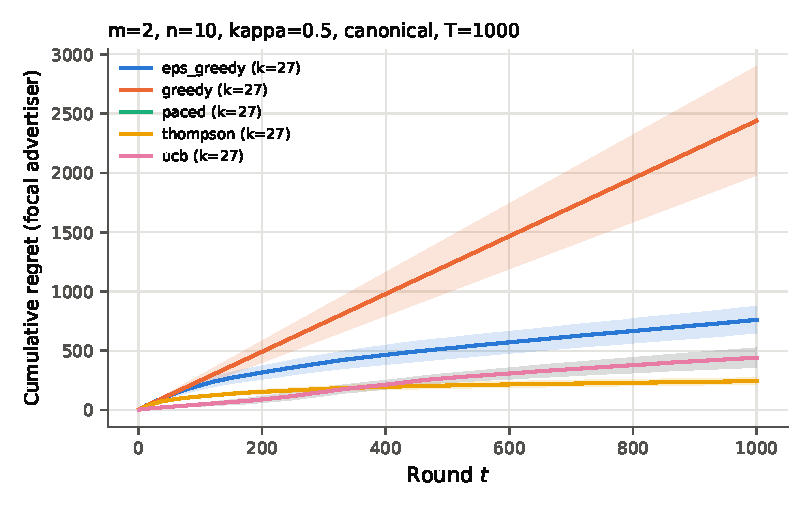
\includegraphics[width=\linewidth]{figures/tier2_curves_cum_regret.pdf}\\[-0.3em]
  {\small (a) Tier 2: cumulative regret of the learner}
\end{minipage}\hfill
\begin{minipage}[t]{0.495\linewidth}\centering
  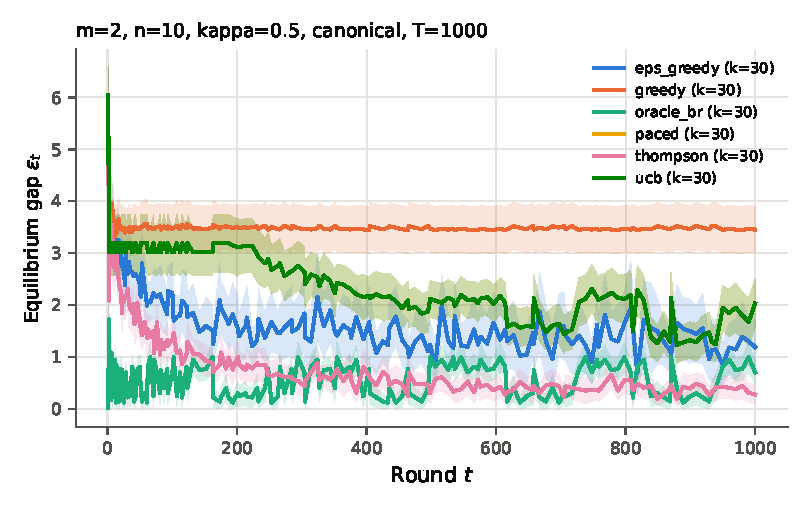
\includegraphics[width=\linewidth]{figures/tier3_curves_eq_gap.pdf}\\[-0.3em]
  {\small (b) Tier 3: equilibrium gap $\varepsilon_t$}
\end{minipage}
\caption{Learning curves for $m=2$, $n=10$, $\kappa=0.5$, canonical budgets; mean and $95\%$ band over
$30$ seeds. In (b), \texttt{oracle\_br} is the known-$f$ best-response control.}
\label{fig:curves}
\end{figure}

\paragraph{H3 is not supported in its proposed form.} Tighter budgets do not slow learning. TS's
regret per round is flat in $\kappa$ ($0.45$--$0.53$), and UCB's \emph{grows} with $\kappa$, from $0.81$ at
$\kappa=0.25$ to $3.38$ at $\kappa=1$, because a larger budget lets an optimistic learner buy more
exploratory impressions each round. The efficiency loss at small $\kappa$ (Table~\ref{tab:t1}) is a
property of the equilibrium and is present before any learning.

\paragraph{Tier 3 (H2): concurrent learning keeps the market away from $b^*$.} Table~\ref{tab:t3}
reports the final state when every advertiser learns. The equilibrium gap grows with $m$ for every
learner, as H2 predicts. The control row shows how much of this is due to learning. Even with known $f$,
simultaneous best response does not settle on $b^*$. It cycles, because each advertiser
reacts to bids that the others are changing in the same round, and its final gap is
$0.76/1.42/2.37$ for $m=2/3/5$. TS ends slightly \emph{closer} to equilibrium than this control
($0.67/1.25/2.48$): random posterior samples desynchronise the advertisers' reactions and damp the
cycling. UCB and $\epsilon$-greedy stay $2$--$5$ units away, and greedy locks into a wrong
profile with efficiency $0.29$. With TS the price of learning is small: efficiency falls by $0.02$ and
revenue by $2.6$ per round, while advertisers' total profit \emph{rises} by $0.3$, since concurrent
bidding competes prices down (the control shows the same pattern). At $T=10^4$ the gap keeps
shrinking for TS ($0.40\to0.29$ at $m=2$, $n=10$) and UCB ($1.64\to0.77$), but not for greedy, so
convergence towards $b^*$ is slow but real for learners whose exploration decays.
\textbf{H2 is supported}, with the qualification that concurrent adaptation alone already produces most of the gap.

\begin{table}[t]
\centering\small
\caption{Tier 3 (all advertisers run the same learner), canonical budgets, $T=10^3$: final-window
equilibrium gap by $m$, and price of learning (Tier-1 value minus final value; positive is a loss)
averaged over the grid. The Tier-1 reference has efficiency $0.58$ and revenue $18.9$ per round.}
\label{tab:t3}
\begin{tabular}{@{}lccccccc@{}}
\toprule
 & \multicolumn{3}{c}{Final gap $\varepsilon$} & & \multicolumn{3}{c}{Price of learning}\\
\cmidrule{2-4}\cmidrule{6-8}
Learner & $m=2$ & $m=3$ & $m=5$ & & Efficiency & Revenue & Total profit\\
\midrule
Known-$f$ best response (control) & $0.76$ & $1.42$ & $2.37$ & & $0.04$ & $4.0$ & $-0.5$\\
Thompson sampling & $\mathbf{0.67}$ & $\mathbf{1.25}$ & $2.48$ & & $\mathbf{0.02}$ & $\mathbf{2.6}$ & $-0.3$\\
UCB, $\alpha=0.5$ & $1.21$ & $2.38$ & $4.04$ & & $0.14$ & $3.0$ & $3.9$\\
UCB, $\alpha=2$ & $2.32$ & $3.67$ & $4.93$ & & $0.23$ & $2.8$ & $7.7$\\
$\epsilon$-greedy & $2.17$ & $3.36$ & $4.82$ & & $0.12$ & $3.3$ & $3.2$\\
Greedy & $4.79$ & $4.82$ & $4.42$ & & $0.29$ & $9.9$ & $4.5$\\
\bottomrule
\end{tabular}
\end{table}

\paragraph{Robustness to the budget structure.} The discounted variant ($\gamma=0.999$) puts more weight on
early rounds but changes no conclusion. TS again wins all $47$ Tier-2 cells, with exponents $0.25$ (TS),
$0.51$ ($\epsilon$-greedy), $0.59$ (UCB) and $0.63$ (greedy). Under a \emph{cumulative} campaign budget
the ranking changes. A myopic learner spends as if the budget reset every round and exhausts it in about half
the horizon. The paced agent has the lowest regret exponent against the fluid benchmark in Tier~2
($2.7$, against $5.8$--$24.6$ for the myopic learners) and the lowest mean regret ($1378$, against
$2912$ for UCB). TS still has the lowest regret in $26$ of $47$ cells. In Tier~3 the paced agent has the
smallest final gap ($2.52/3.21/3.89$ for $m=2/3/5$, against $4.1$--$5.0$ for TS) and the smallest
revenue loss ($5.9$ against $10$--$13$). With one campaign budget, pacing matters more than the choice
of bandit index. Under per-round budgets the paced agent's dual price stays at $0$, and it behaves
exactly like UCB.

% =====================================================================
\section{Discussion and limitations}
Three findings stand out. First, \emph{learning against a fixed market is cheap}. With posterior
sampling, regret grows roughly logarithmically, and over $10^3$ rounds the learner earns on average
within about $8\%$ of its best-response profit ($0.49$ regret against $5.78$ profit per round). The knapsack oracle does the combinatorial work, and the bandit index only has to
rank users. Second, \emph{concurrent adaptation, not learning, is the main obstacle to equilibrium}.
Known-$f$ best response cycles, so the Tier-3 gap is mostly a property of the dynamics. Randomised
learners can even reduce it. Third, \emph{budget scarcity acts through the equilibrium}. Tight
budgets leave users unallocated or misallocated at $b^*$ itself. They do not make learning slower, and
an optimistic learner with more budget spends more of it on exploration.

\paragraph{Limitations.} (i) Integer bids force $v=5$. A finer bid grid would change the knapsack
weights and possibly the equilibria. (ii) Tier-2 excludes instances without a pure equilibrium, which
makes the large-$m$, large-$n$ cells rest on fewer seeds (excluded counts are reported per cell in the
supplement). (iii) The paper's Assumption~2 reveals the highest competing bid. With win/loss feedback
only, the learner would also have to estimate the price of each user. (iv) Instances are synthetic,
with independent Beta click rates. Real click rates are correlated across users and advertisers.

% =====================================================================
\section{Conclusion and future work}
A batched first-price auction with budgets reduces, round by round, to a knapsack problem under
uncertainty. Coupling an exact knapsack oracle with Thompson sampling gives sublinear regret against a
stationary market (H1). When every advertiser learns, the market stays near, but not at, the
equilibrium, and the distance grows with the number of advertisers (H2). Scarce budgets hurt efficiency
through the equilibrium, not through slower learning (H3 rejected as stated). Following the TA's
feedback we kept the scope to the three tiers. The two most direct extensions are contextual click
models that share information across similar users through features (a LinUCB-style
index~\citep{li2010contextual}), and learning the winning-price distribution from win/loss
outcomes alone.

\paragraph{Reproducibility and live demo.}\label{sec:repro} All code, sweep outputs and figures are
in the repository. \texttt{python run\_tests.py} runs the $54$ tests for all tiers, the harness and the demo;
\texttt{python run\_evaluation.py sweep \dots} followed by \texttt{report} regenerates every table and
figure (commands in the README and supplement). \texttt{python run\_demo.py} animates a market round by
round with the project's own agents, showing bids, wins, clicks, learned versus true click rates, regret,
equilibrium gap and efficiency. \texttt{demo/index.html} is a browser version of the same demo that
needs no installation.

\paragraph{Contributions.} Vivek Raj: Tier-1 knapsack DP, equilibrium solvers and social planner.
Anvit Aggarwal: Tier-2 learners (UCB, TS, greedy, $\epsilon$-greedy, budget-paced). Eshaan Ashish
Jaiswal: Tier-3 multi-agent simulator and convergence analysis. Gella Naga Sai Krishna: evaluation
harness, sensitivity study, live demo, report and presentation.

\small
\begin{thebibliography}{9}
\bibitem{badanidiyuru2013bandits}
A.~Badanidiyuru, R.~Kleinberg, and A.~Slivkins.
\newblock Bandits with knapsacks.
\newblock In \emph{Proc.\ FOCS}, 2013.

\bibitem{agrawal2014bandits}
S.~Agrawal and N.~R.~Devanur.
\newblock Bandits with concave rewards and convex knapsacks.
\newblock In \emph{Proc.\ ACM EC}, 2014.

\bibitem{chen2013combinatorial}
W.~Chen, Y.~Wang, and Y.~Yuan.
\newblock Combinatorial multi-armed bandit: General framework and applications.
\newblock In \emph{Proc.\ ICML}, 2013.

\bibitem{li2010contextual}
L.~Li, W.~Chu, J.~Langford, and R.~E.~Schapire.
\newblock A contextual-bandit approach to personalized news article recommendation.
\newblock In \emph{Proc.\ WWW}, 2010.
\end{thebibliography}

\end{document}
